% Options for packages loaded elsewhere
\PassOptionsToPackage{unicode}{hyperref}
\PassOptionsToPackage{hyphens}{url}
%
\documentclass[
  12pt,
]{article}
\usepackage{amsmath,amssymb}
\usepackage{iftex}
\ifPDFTeX
  \usepackage[T1]{fontenc}
  \usepackage[utf8]{inputenc}
  \usepackage{textcomp} % provide euro and other symbols
\else % if luatex or xetex
  \usepackage{unicode-math} % this also loads fontspec
  \defaultfontfeatures{Scale=MatchLowercase}
  \defaultfontfeatures[\rmfamily]{Ligatures=TeX,Scale=1}
\fi
\usepackage{lmodern}
\ifPDFTeX\else
  % xetex/luatex font selection
\fi
% Use upquote if available, for straight quotes in verbatim environments
\IfFileExists{upquote.sty}{\usepackage{upquote}}{}
\IfFileExists{microtype.sty}{% use microtype if available
  \usepackage[]{microtype}
  \UseMicrotypeSet[protrusion]{basicmath} % disable protrusion for tt fonts
}{}
\makeatletter
\@ifundefined{KOMAClassName}{% if non-KOMA class
  \IfFileExists{parskip.sty}{%
    \usepackage{parskip}
  }{% else
    \setlength{\parindent}{0pt}
    \setlength{\parskip}{6pt plus 2pt minus 1pt}}
}{% if KOMA class
  \KOMAoptions{parskip=half}}
\makeatother
\usepackage{xcolor}
\usepackage[margin=1in]{geometry}
\usepackage{graphicx}
\makeatletter
\def\maxwidth{\ifdim\Gin@nat@width>\linewidth\linewidth\else\Gin@nat@width\fi}
\def\maxheight{\ifdim\Gin@nat@height>\textheight\textheight\else\Gin@nat@height\fi}
\makeatother
% Scale images if necessary, so that they will not overflow the page
% margins by default, and it is still possible to overwrite the defaults
% using explicit options in \includegraphics[width, height, ...]{}
\setkeys{Gin}{width=\maxwidth,height=\maxheight,keepaspectratio}
% Set default figure placement to htbp
\makeatletter
\def\fps@figure{htbp}
\makeatother
\setlength{\emergencystretch}{3em} % prevent overfull lines
\providecommand{\tightlist}{%
  \setlength{\itemsep}{0pt}\setlength{\parskip}{0pt}}
\setcounter{secnumdepth}{5}
\usepackage{setspace,lscape} \usepackage{amsmath} \usepackage{array} \usepackage{caption,subcaption} \usepackage{longtable} \usepackage{booktabs} \usepackage{enumitem} \usepackage{standalone} \renewcommand{\arraystretch}{1.5} \captionsetup[table]{skip=5pt} \setstretch{1.5}
\ifLuaTeX
  \usepackage{selnolig}  % disable illegal ligatures
\fi
\usepackage[]{natbib}
\bibliographystyle{apalike}
\IfFileExists{bookmark.sty}{\usepackage{bookmark}}{\usepackage{hyperref}}
\IfFileExists{xurl.sty}{\usepackage{xurl}}{} % add URL line breaks if available
\urlstyle{same}
\hypersetup{
  pdftitle={Results of Experiment 2},
  pdfauthor={Zijian Zark Wang},
  hidelinks,
  pdfcreator={LaTeX via pandoc}}

\title{Results of Experiment 2}
\author{Zijian Zark Wang}
\date{February 22, 2024}

\begin{document}
\maketitle

\hypertarget{sample}{%
\section{Sample}\label{sample}}

Each subject was required to complete a survey. The survey contains 14
fill-in-the-blank questions as the main task, 4 choice questions for
consistency check, and one additional choice question for measuring
impatience.

In each fill-in-the-blank question, participants will face two options -
Option A and Option B - framed as sequences of rewards. Option A offers
two rewards at two specific times: one reward is delivered today and the
other is delivered after a certain delay (e.g.~``receive £185 today and
£60 in 6 months''). Option B offers an unknown amount today and no
amount after the same delay. Participants have to identify which level
of this unknown amount would make them value the two options equally,
and fill in their answer in a box. Figure \ref{fig:fill-blank-screen}
presents an example question. Throughout the survey, the delayed amount
in Option A is fixed at £60. We set up two levels for the delay (6
months and 12 months) and seven levels for the amount offered today
(£25, £105, £185, £265, £345, £425, £505) in Option A. Overall, there
are 14 fill-in-the-blank questions, presented in a random order.

\begin{figure}
  \vspace{16pt}
  \centering
  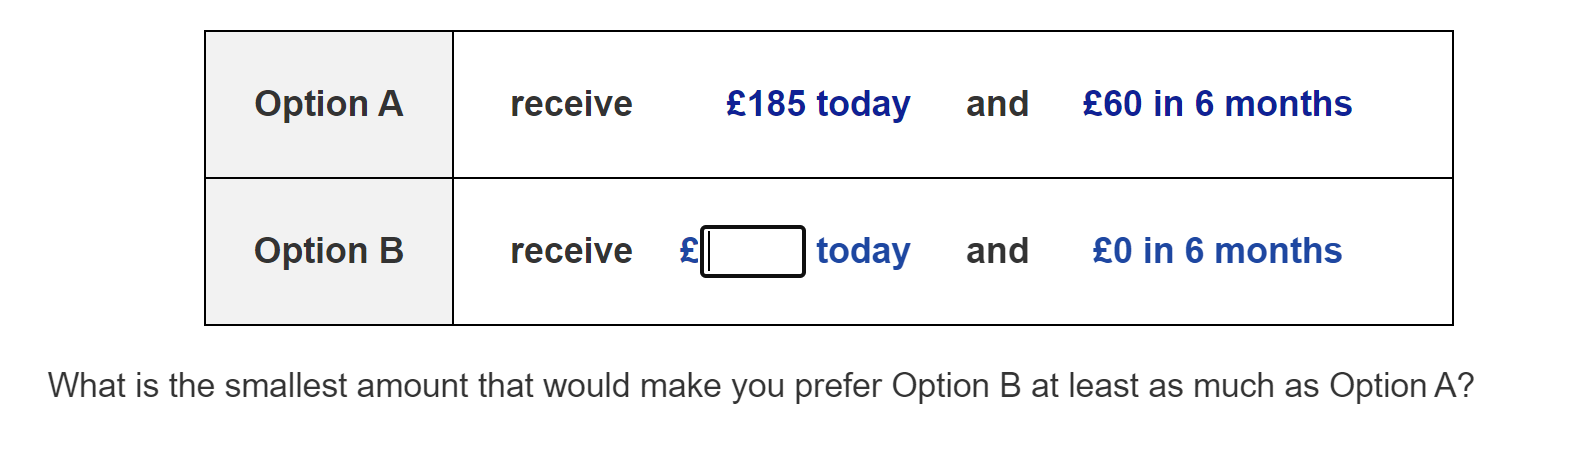
\includegraphics[width=0.96\textwidth]{figures/screenshot.png}
  \caption{Screenshot of An Fill-in-the-Blank Question}
  \label{fig:fill-blank-screen}
\end{figure}

Before participants start doing the main task, there are four
consistency check questions. Each consistency check question contains
two options: one is the same as Option A in a subsequent
fill-in-the-blank question; the other offers a specific amount today and
no amount in the future. In the latter option, the amount offered today
is either the same as that of the former option, or above the total
money in the former option. Participants are required to choose the
option they prefer. We exclude the participants whose choices are
inconsistent with their answers in the corresponding fill-in-the-blank
questions. For example, a participant may face a choice between
``receive £185 today and £60 in 6 months'' and ``receive £300 today and
£0 in 6 months''. If she chooses the latter option, then for a
fill-in-the-blank question setting the former option as Option A, she
should fill in an amount smaller than £300. Finally, at the end of the
survey, we add one additional question to measure impatience. The
question is the same as the ``Preference for Earlier vs Later Income''
(PELI) task in \citet{burro2022patience}.

Two hundred subjects (female: 50\%) were recruited via Prolific, of
which 197 subjects completed the survey\footnote{When a question was
  loaded multiple times during the survey completion process, the survey
  will be automatically ended and submitted, in order to prevent
  duplicate responses. This situation occurred with three participants.
  We thus abort their answers.}. The median age for those who completed
the survey is 38, the median completion time is 4.8 minutes. The minimum
completion time is 1.83 minutes. We offer £1.2 for each participant.
There were 161 subjects having passed the consistency check. Given that
each subject completed 14 fill-in-the-blank questions, we construct a
sample of 2,254 observations.

\hypertarget{theoretical-analysis}{%
\section{Theoretical Analysis}\label{theoretical-analysis}}

Before diving into the results, it is helpful to know some notation and
terms about the main task. Suppose in a question, Option A is ``receive
\(Y_1\) today and \(Y_2\) in delay \(T\)'', and a subject values this
option A equally as much as ``receive \(M\) today and £0 in delay
\(T\)'' (Option B). \(Y_1\) is the front-end amount of the sequence,
\(Y_2\) is the back-end amount, \(T\) is the sequence length, and the
answer \(M\) is termed the ``indifference point'' between the two
options. It is revealed that the subject values the back-end amount
\(Y_2\) (fixed throughout the survey) in Option A at the same level as
receiving \(M - Y_1\) today in Option B. So, we also term \(M - Y_1\) as
the revealed value of that back-end amount. We focus on how \(M - Y_1\)
varies with \(Y_1\).

One popular way to model this decision is through additive discounted
utilities, that is, \(M\) is determined by\[
u(M) = u(Y_1) + D_T \cdot u(Y_2)
\]where \(u(.)\) is a strictly concave utility function and \(D_T\) is
the discount factor of the reward delivered in delay \(T\). As many
models of this type (e.g.~hyperbolic discounting) assumes, in the case
that \(T\) and \(Y_2\) are both constant, the term \(D_T\cdot u(Y_2)\)
should also be constant, which implies the value of \(u(M) - u(Y_1)\)
should be constant for the equation to be true. Given that \(u(.)\) is
strictly concave, for any positive real number \(\Delta\), we must have
\(u(M+\Delta) - u(Y_1 + \Delta) > u(M) - u(Y_1)\). That is, when \(Y_1\)
is increased by \(\Delta\) units, to make the equation hold, \(M\)
should be increased by an amount larger than \(\Delta\). Therefore, many
models of this type predict \(M - Y_1\) is increasing in \(Y_1\).

It is notable that the concavity of utility function implies
\(u(Y_1 + Y_2) < u(Y_1) + u(Y_2)\). Hence, when \(D_T\) is large enough,
it is possible that \(M\) becomes an amount greater than \(Y_1 + Y_2\)
for the equation to be true.

My prediction about the results is as follows. When the front-end amount
\(Y_1\) is increased, people would pay more attention to \(Y_1\). Given
their attention is limited, the back-end amount \(Y_2\) receives less
attention, which means people take into less account the back-end amount
when valuing the whole sequence. As a results, the revealed value of the
back-end amount could decrease with the front-end amount, i.e.~\(M-Y_1\)
could decrease in \(Y_1\).

\hypertarget{heterogeneity-in-responses}{%
\section{Heterogeneity in Responses}\label{heterogeneity-in-responses}}

The left side of Figure \ref{fig:response_dist} illustrates the
distribution of indifference points for each question. The y-axis of
this subfigure indicates \(M - Y_1\), i.e.~the revealed value of the
back-end amount (£60) in Option A. 86.4\% of the observations fall
within the range of £0 to £60; 12.8\% of the observations are above £60,
which implies the participants value Option A as much as receiving an
amount greater than its total money today; 0.8\% of the observations is
negative, indicating that the participants value Option A as much as
receiving an amount lower than its front-end amount today. The latter
two could originate from various causes, e.g.~participants made mistakes
or over-rounded when filling in answers. Some observations in these two
cases should be viewed as outliers. For example, the maximum and minimum
revealed values of the back-end amount are £375 and -£265.\footnote{For
  the maximum case, the participant values ``receive £425 today and £60
  in 12 months'' as much as receiving £800 today, but values ``receive
  £505 today and £60 in 6 months'' as much as receiving £505 today. For
  the minimum case, the participant values ``receive £425 today and £60
  in 12 months'' as much as receiving £160 today, but for all the other
  questions, the revealed value of the back-end amount is ranged between
  £15 and £60. Thus, it is likely that such observations are mistakes.}

We analyze the data and deal with the outliers in three ways. First, we
use non-parametric methods (rank correlation) for a preliminary measure
of the relationship between \(M - Y_1\) and \(Y_1\). Second, we examine
the relationship between \(M - Y_1\) and \(Y_1\) in regressions. In OLS
regressions, we remove the 12 most extreme observations. These
observations account for about 0.5\% of the entire sample and removing
them would have no substantial effect over the sample distribution.
Finally, we conduct robust regressions over the entire sample (without
removing any outlier). Given that robust estimators are generally
insensitive to outliers, we suggest the readers prioritize results of
the robust regressions where possible.

Meanwhile, a substantial fraction of observations (43.8\%) are simply
\(Y_1 + Y_2\), i.e.~the total money to be obtained in Option A. The
right side of Figure \ref{fig:response_dist} illustrate the distribution
of such observations over the participants. Overall, 62 participants
(38.5\% of all participants who gave valid answers) used total money to
answer every question; on the contrary, 65 participants have never used
total money. This suggests that different people used different ways to
value the sequence Option A, and one of those ways is to value a reward
sequence purely by its total money.

The ``total money'' answers are highly likely to be a heuristic because
on average these answers take less time (9.28s) than the other answers
(10.88s), and the difference is significant (two-sample test: \(t\) =
4.177, \(p\)-value = \(3.06\times10^{-5}\)).

\begin{figure}
    \centering
    \begin{subfigure}{0.5\textwidth}
        \centering
        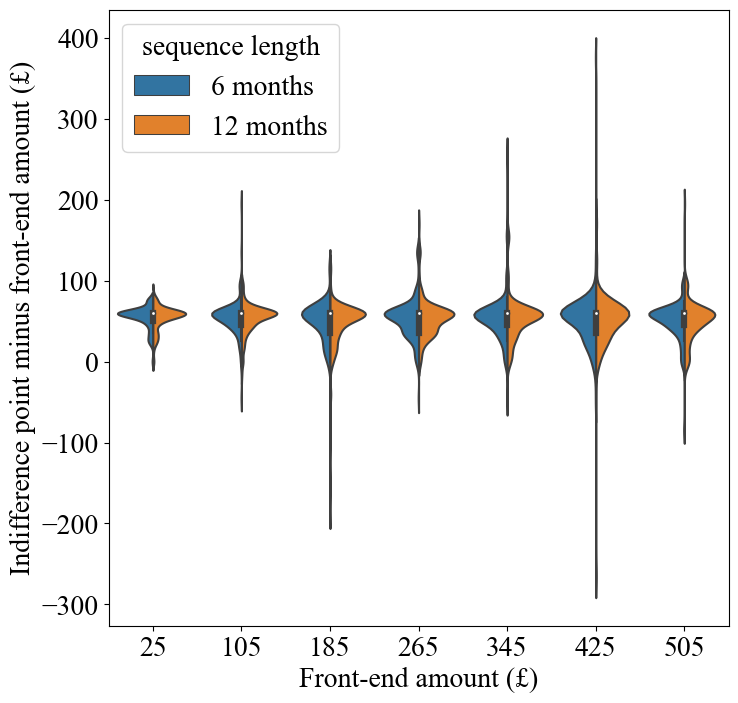
\includegraphics[width=\linewidth]{figures/outlier.png} 
    \end{subfigure}
    \hfill
    \begin{subfigure}{0.49\textwidth}
        \centering
        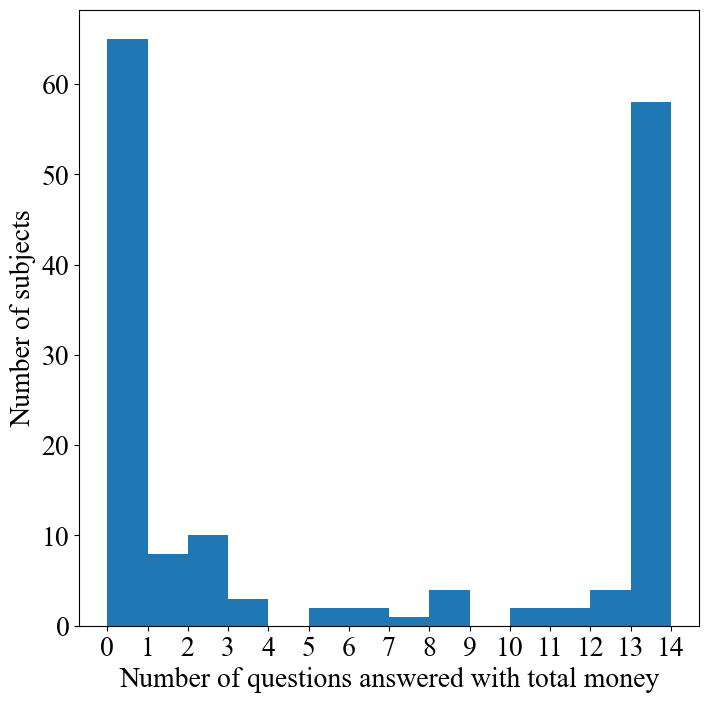
\includegraphics[width=\linewidth]{figures/total_money.png} 
    \end{subfigure}
    \caption{Distribution of Responses}
    \label{fig:response_dist}
\end{figure}

To identify the ways of valuing that people used in the main task, we
use k-means clustering method to analyze their answers over all
fill-in-the-blank questions, and divide the participants who gave valid
answers into two groups. The first group (cluster 1) has 104
participants, and the second (cluster 2) has 57 participants.\footnote{In
  the case that there are three clusters, the number of participants in
  each cluster is 105, 55 and 1. In the case of four clusters, the
  number of participants in each cluster is 105, 46, 1 and 9. We only
  divide people into two groups because the size for the third (and
  fourth) group is too small.} The Mann-Whitney U test rejects the
hypothesis that the two clusters are drawn from a same population (\(U\)
= 1059304.0, \(p\)-value = \(2.67 \times 10^{-251}\)).

The proportion of the ``total money'' answers is 63.1\% in cluster 1,
and is only 8.6\% in cluster 2, and the difference is significant
(Pearson's \(\chi^2 = 619.040\), \(p\)-value =
\(1.21\times 10^{-136}\)). Over 79\% of the observations in cluster 2
are above £0 and lower than £60. Thus, people in cluster 1 are more
likely to use total money to value a reward sequence, while those in
cluster 2 are more likely to value the back-end amount through a delay
discounting approach.

Figure \ref{fig:cluster_result} shows the median and mean revealed
values of the back-end amount £60 for each question. The patterns of
lines in Figure \ref{fig:cluster_result} also suggest that people in
cluster 1 tend to use the total money in answers, while for people in
cluster 2, an increase in the front-end amount \(Y_1\) tends to reduce
the revealed value of the back-end amount, i.e.~\(M - Y_1\).

\begin{figure}
    \centering
    \begin{subfigure}{0.51\textwidth}
        \centering
        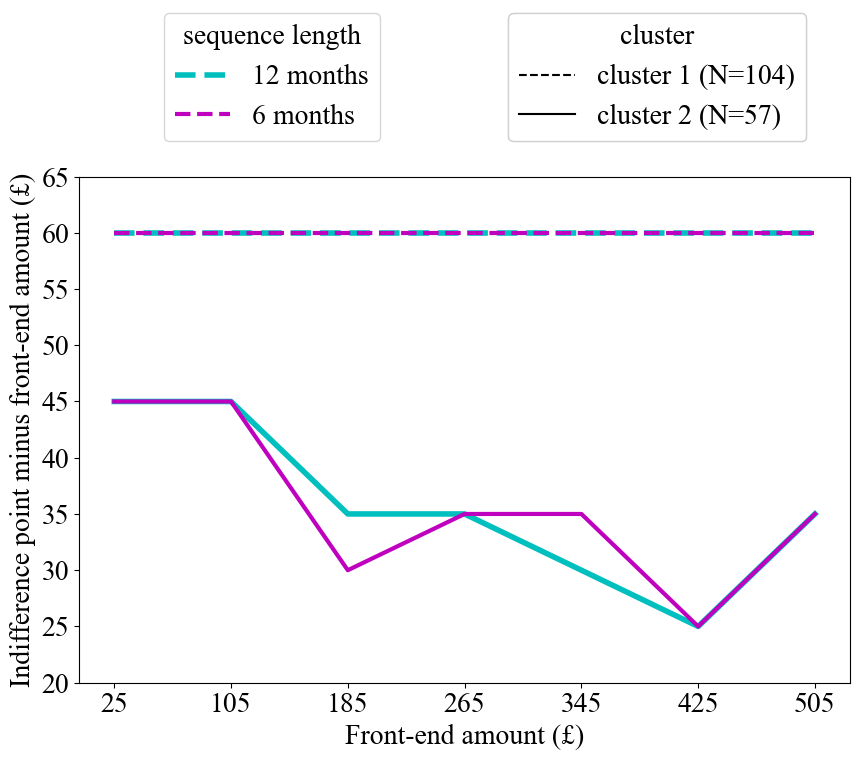
\includegraphics[width=\linewidth]{figures/cluster_result_median.png} 
        \caption{median}
    \end{subfigure}
    \hfill
    \begin{subfigure}{0.48\textwidth}
        \centering
        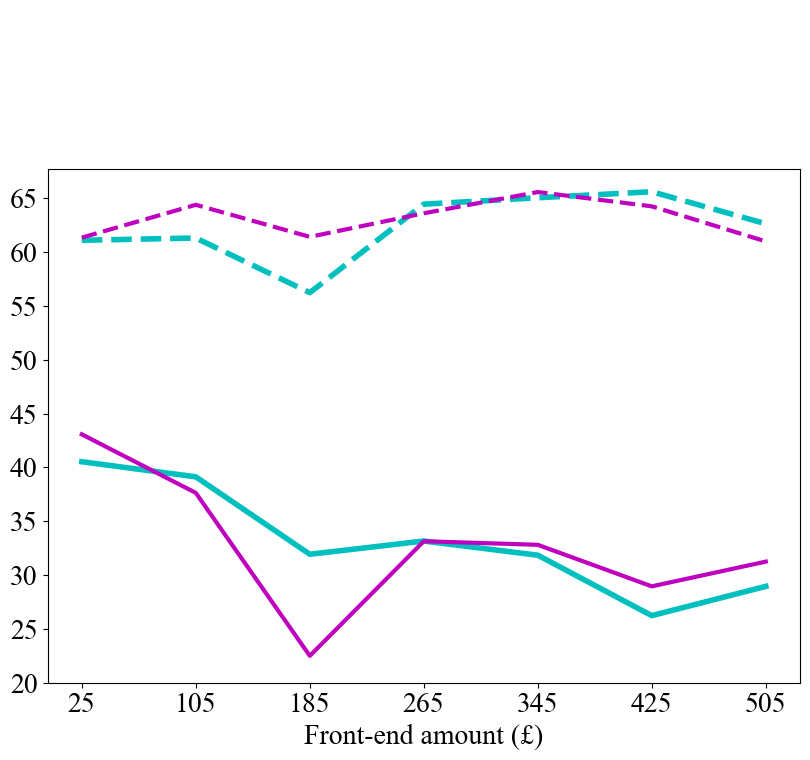
\includegraphics[width=\linewidth]{figures/cluster_result_mean.png}
        \caption{mean}
    \end{subfigure}
    \caption{Median and Mean Indifference Point minus the Front-End Amount in Each Fill-in-the-Blank Question}
    \label{fig:cluster_result}
\end{figure}

\hypertarget{regression-results}{%
\section{Regression Results}\label{regression-results}}

We first look at the rank correlation coefficients. The Spearman's
\(\rho\) between \(M - Y_1\) and \(Y_1\) is -0.049, which indicates a
weak negative correlation between the back-end amount's revealed value
and the front-end amount (\(p\)-value = 0.021). For people in cluster 1,
the Spearman's \(\rho\) is -0.015 (\(p\)-value = 0.556); for people in
cluster 2, the Spearman's \(\rho\) is -0.189 (\(p\)-value =
\(7.19\times 10^{-8}\)). This indicates that the revealed value of the
back-end amount in cluster 1 is irrelevant to the front-end amount,
while that in cluster 2 is significantly decreasing with the front-end
amount.

An analysis based on other statistics yields similar results. The
Kendall's \(\tau\) between \(M-Y_1\) and \(Y_1\) is -0.038 (\(p\)-value
= 0.018). For people in cluster 1, the Kendall's \(\tau\) is -0.013
(\(p\)-value = 0.552); for people in cluster 2, the Kendall's \(\tau\)
is -0.148 (\(p\)-value = \(2.56\times 10^{-8}\)).

We then run linear regressions. The back-end amount's revealed value
\(M- Y_1\) is set as the dependent variable, and independent variables
are the front-end amount \(Y_1\) under each sequence length \(T\), and
the participants' responses to the PELI question (hereinafter referred
to as PELI). The variable PELI is 1 if a participant chooses the large
later income and 0 if she chooses the small earlier income. Meanwhile,
we use variables CL1 and CL2 to represent clustering results. The
variable CL1 is 1 if a participant is in cluster 1 and 0 otherwise; the
variable CL2 is 1 if a participant is in cluster 2 and 0 otherwise. To
examine individual heterogeneity in responses, we construct interaction
variables between the clustering results and \(Y_1\). The coefficients
for these interactions reflect how participants in each clusters react
differently to the variation of \(Y_1\) under each sequence length
\(T\). Table \ref{tab:seq_value_reg} illustrates the regression results.


\documentclass[12pt]{article}


\begin{document}
\begin{table}
    \caption{Regression Results}
    \vspace*{12pt}
    \centering

      \begin{tabular}{lllllll}
\hline
 & (1) Pool & (2) Pool & (3) FE & (4) FE & (5) RLM & (6) RLM \\
\hline
$Y_1\cdot1\{T=T_L\}$ & -0.005$^{**}$ &  & -0.005$^{*}$ &  & -0.005$^{***}$ &  \\
 & (0.002) &  & (0.002) &  & (0.001) &  \\
$Y_1\cdot1\{T=T_H\}$ & -0.006$^{***}$ &  & -0.005$^{**}$ &  & -0.006$^{***}$ &  \\
 & (0.002) &  & (0.002) &  & (0.001) &  \\
$Y_1\cdot1\{T=T_L\}\times$CL1 &  & 0.022$^{***}$ &  & 0.002 &  & 0.0 \\
 &  & (0.004) &  & (0.002) &  & (0.001) \\
$Y_1\cdot1\{T=T_H\}\times$CL1 &  & 0.023$^{***}$ &  & 0.003 &  & -0.0 \\
 &  & (0.004) &  & (0.002) &  & (0.001) \\
$Y_1\cdot1\{T=T_L\}\times$CL2 &  & -0.06$^{***}$ &  & -0.019$^{***}$ &  & -0.017$^{***}$ \\
 &  & (0.005) &  & (0.004) &  & (0.002) \\
$Y_1\cdot1\{T=T_H\}\times$CL2 &  & -0.062$^{***}$ &  & -0.021$^{***}$ &  & -0.022$^{***}$ \\
 &  & (0.005) &  & (0.004) &  & (0.002) \\
PELI & -0.239 & -0.645 & 9.187$^{***}$ & 7.215$^{***}$ & 2.181$^{***}$ & 2.206$^{***}$ \\
 & (3.95) & (2.638) & (0.015) & (0.364) & (0.319) & (0.31) \\
Constant & 53.742$^{***}$ & 54.037$^{***}$ & 46.434$^{***}$ & 47.965$^{***}$ & 52.158$^{***}$ & 52.385$^{***}$ \\
 & (3.619) & (2.684) & (0.485) & (0.432) & (0.361) & (0.351) \\\hline

observations & 2186 & 2186 & 2186 & 2186 & 2198 & 2198 \\
adj-$R^2$ & 0.0 & 0.334 & 0.648 & 0.654 &  &  \\
Muller-Welsh &  &  &  &  & 128.457 & 122.183 \\
\hline
\end{tabular}
% INSERT reg_combined

    \vspace*{4pt}
    \centering
    \begin{minipage}{1.0\textwidth}
    {\par\footnotesize Note: * $p<0.05$, ** $p<0.01$, *** $p<0.001$. Standard errors are reported in the parentheses. Model (1)-(2) are pooled OLS models, model (3)-(4) are fixed-effect OLS models, model (5)-(6) are fixed-effect robust linear regressions (RLM). For OLS, standard errors are clustered at the subject level, and p-values are calculated using t-tests. For RLM, each model is estimated using Huber's M-estimator (the threshold for loss function is set at 1.345) and the scale estimator is Huber's proposal 2 estimator. Each p-value for RLM is calculated based on a normal distribution with i.i.d. assumption. A smaller Muller-Welsh score indicates the model has a greater ability to both parsimoniously fit the data and predict new independent obeservations. $Y_1$ and $T$ denote the front-end amount and the sequence length in Option A. $T_L$ and $T_H$ are 6 months and 12 months, respectively. Clustering results are obtained through k-means method.}
    \end{minipage}
    \label{tab:seq_value_reg}
\end{table}

\end{document}



The main results are illustrated by column (3)-(6) in Table
\ref{tab:seq_value_reg}. These columns are models with individual fixed
effects. Column (3)-(4) are the OLS regressions run after removing 12
outliers; column (5)-(6) are the robust regressions run on the entire
sample. For robust regressions, we use Huber's M-estimator for loss
function and use Huber's proposal 2 estimator for scale estimator.
Results produced by this robust method are less sensitive to outliers
than the OLS estimator \citep{huber2009robust}. Under each estimator,
these fixed-effect models yield similar results: First, the revealed
value of back-end amount is overall slightly decreasing with the
front-end amount. Second, for people in cluster 1, an increase in
front-end amount has no impact on how people value the back-end amount.
But for those in cluster 2, this significantly reduces the revealed
value of the back-end amount (\(p\)-value \textless{} 0.005). Notablely,
according to column (6), for people in cluster 2, an £100 increase in
the front-end amount reduces the revealed value of the back-end amount
by £1.8 when the sequence is 6-month long, and by £2.2 when the sequence
is 12-month long, which are 3.0\% and 3.7\% of the amount £60.

In addition, column (1)-(2) in Table \ref{tab:seq_value_reg} are the
pooled OLS regressions run after removing outliers. The adjusted \(R^2\)
for column (1)-(2) indicates that incorporating clustering results in
such model can improve the goodness of fit by a lot (from 0.001 to
0.335). For robust regressions, we use the Muller-Welsh criterion to
measure the model performance \citep{muller2005outlier}. The model
incorporating clustering results possesses a smaller Mull-Welsh score,
which means it performs a greater ability to parsimoniously fit the data
and predict new independent observations than the other
model\footnote{The calculation of the Muller-Welsh criterion requests
  applying stratified bootstrap. To construct bootstrap samples, we
  divide observations into three strata (the upper tail, the lower tail,
  the others), and draw observations with replacement within each
  stratum. Each bootstrap sample is 50\% in size of the entire sample,
  and the process is repeated 1,000 times.}.

\hypertarget{discussion}{%
\section{Discussion}\label{discussion}}

\hypertarget{estimating-the-confidence-intervals}{%
\subsection{Estimating the confidence
intervals}\label{estimating-the-confidence-intervals}}

One may argue that the residuals in regressions are not normally
distributed due to the existence of outliers. In such cases, conducting
hypothesis testing based on the normality assumption may be
inappropriate. Thus, we obtain the confidence intervals for regression
coefficients via a stratified bootstrap method. Figure
\ref{fig:bootstrap_ci} illustrate the bootstrap 95\% confidence
intervals for key fixed-effect estimates in column (5)-(6) of Table
\ref{tab:seq_value_reg}. The results in Table \ref{tab:seq_value_reg}
remain robust to this bootstrap method: overall, the revealed value of
the back-end amount slightly decreases with the front-end amount; the
front-end amount has no impact on the value of the back-end amount for
cluster 1 but has a negative effect for cluster 2.

\begin{figure} 
\centering
\begin{subfigure}{0.85\textwidth}
  \hfill
  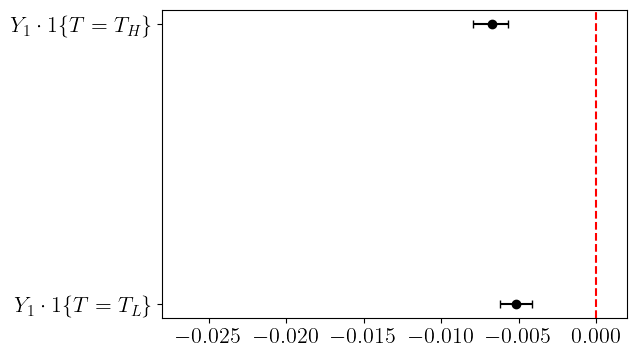
\includegraphics[width=0.85\linewidth]{figures/bootstrap_ci_baseline.png}
\end{subfigure}
\begin{subfigure}{0.85\textwidth} 
  \hfill
  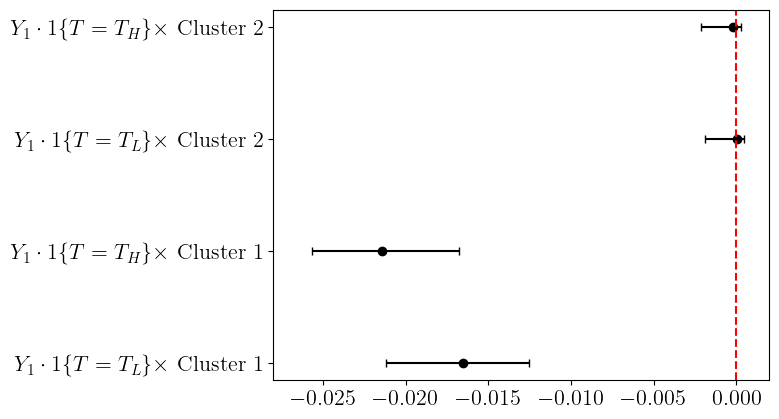
\includegraphics[width=\linewidth]{figures/bootstrap_ci_label.png} 
\end{subfigure}
\caption{Bootstrap 95\% Confidence Intervals for the Fixed-Effect Estimates in Robust Regressions}
\vspace*{4pt}
\centering
\begin{minipage}{1.0\textwidth}
{\par\footnotesize Note: The subfigures on the top and the bottom correspond to column (5) and (6) in Table \ref{tab:seq_value_reg} respectively. The dots are the original estimates and the error bars indicate the confidence intervals. To approximate the distribution for each coefficient, we use the stratified bootstrap method. The observations are divided into three strata based on RLM results: the upper tail (with high residuals and a weight of 1), the lower tail (with low residuals and a weight of 1), and the others. We draw observations with replacement within each stratum and use them to estimate the coefficients. Each bootstrap sample is the same size as the original sample, and the process is repeated 1,000 times. }
\end{minipage}
\label{fig:bootstrap_ci}
\end{figure}

\hypertarget{responses-to-the-peli-question}{%
\subsection{Responses to the PELI
question}\label{responses-to-the-peli-question}}

The coefficients for PELI in Table \ref{tab:seq_value_reg} are all
significantly positive at significance level 0.5\%. This suggest that
people who are less impatient (choosing the large later income rather
than the small earlier income) tend to value the back-end amount at a
higher level. The Mann-Whitney U test on the revealed value of the
back-end amount also rejects the hypothesis that people who choose
different options in the PELI question value the back-end amount at the
same level (\(U\) = 421520.0, \(p\)-value = 0.004).

The relationship between the PELI and the ways of valuing a sequence is
unclear. Putting the clustering results and the PELI into a contingency
table, we obtain \(\chi^2\) = 0.550 (\(p\)-value = 0.458, df = 1).
However, the result is opposite for a different clustering method. We
classify the 62 participants who use total money to answer every
question into one cluster and the other 99 participants into another,
and construct another contingency table. The contingency table indicates
that those who are less impatient are more likely to use total money to
answer all questions (\(\chi^2\) = 11.063, \(p\)-value = 0.001, df = 1).

\hypertarget{alternative-clustering-methods}{%
\subsection{Alternative clustering
methods}\label{alternative-clustering-methods}}

As a robustness check, we use a Gaussian mixture model to cluster
participants into two groups. The Gaussian mixture model exactly groups
the participants who use total money to answer every question (N=62)
into cluster 1, and groups the remaining 99 participants into cluster 2.
Substituting the clustering results obtained from the Gaussian mixture
model into the regressions gives similar results to the k-means method.
Figure \ref{fig:bootstrap_ci_gmm} illustrates the bootstrap 95\%
confidence intervals for key fixed-effect estimates in a model estimated
using Huber's M-estimator. The model corresponds to column (6) in Table
\ref{tab:seq_value_reg}. The results suggest that increasing the
front-end amount has no effect on the revealed value of the back-end
amount for people in cluster 1 but can significantly reduce it for
people in cluster 2.

\begin{figure} 
\centering
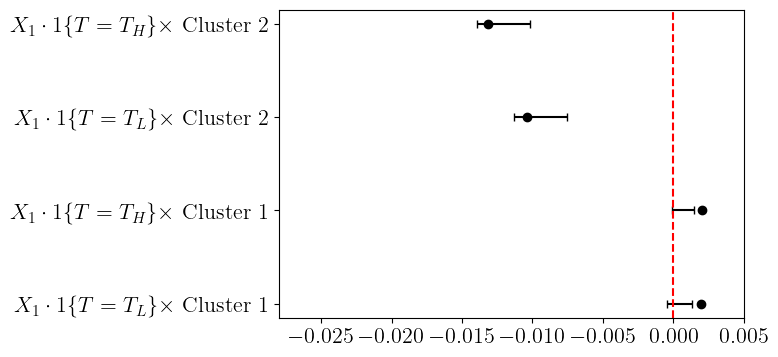
\includegraphics[width=0.85\linewidth]{figures/bootstrap_ci_label_gmm_fe.png}
\caption{Clustering with Gaussian Mixture Model: Bootstrap 95\% Confidence Intervals for the Fixed-Effect Estimates in Robust Regressions}
\vspace*{4pt}
\centering
\begin{minipage}{1.0\textwidth}
{\par\footnotesize Note: The dots are the original estimates and the error bars indicate the confidence intervals.}
\end{minipage}
\label{fig:bootstrap_ci_gmm}
\end{figure}

\hypertarget{alternative-explanations}{%
\subsection{Alternative explanations}\label{alternative-explanations}}

This research examines how people evaluate a two-reward sequence. We
propose that, due to limited attention, an increase in the front-end
amount would make some people discount the value of the back-end amount
to a greater extent.

One alternative explanation to this phenomenon is that, people prefer
increasing sequences to decreasing sequences. Hence, when the front-end
amount is increased, the sequence becomes more ``decreasing''. This lead
people to devalue the whole sequence by a larger degree.

The trade-off theory of intertemporal choice also offers an alternative
explanation\citep{read2012tradeoffs, scholten2023unified}. The theory
propose that, when valuing a sequence of rewards, people would trade off
the total money against the weighted average delay of rewards. For
example, for ``receive \(Y_1\) today and \(Y_2\) in delay \(T\)'', the
average delay of rewards is a weighted sum of 0 and \(T\). Suppose they
value this reward sequence equally with receiving \(M\) today and no
reward at other times. In the trade-off theory, \(M\) is determined by
\(u(M)=u(Y_1+Y_2)- w\cdot T\), where \(w\) is the weight assigned to the
delay \(T\). For simplicity, we do not consider the changes in \(w\).
Given that \(Y_1 + Y_2 > M\) and the utility function \(u(.)\) is
concave, when \(Y_1\) is increased by one unit, \(M\) should increase by
an amount lower than one unit to hold \(u(Y_1 + Y_2) - u(M)\)
constant\footnote{Note the trade-off theory does not allow
  \(M > Y_1 + Y_2\). However, for 12.8\% of the observations, \(M\) is
  larger than \(Y_1 + Y_2\).}.

\renewcommand\refname{Reference}
  \bibliography{experiment-2-ref.bib}

\end{document}
